\subsection{The Fiber TX module} 

The Fiber TX module (figure \ref{fibertx})  formats data for transmission according to the
Soma FiberIO Protocol. All inputs are latched on the
\signal{OUTSAMPLE} signal to prevent word-skew.

The counter \signal{INCNT} counts the assertion of the input
\signal{YEN} to write samples from the output of the RMAC. These are stored in an appropriate array of registers \signal{YL[n]}.

A giant mux controlled by an \signal{OUTBYTE}-enabled counter multiplex the relevant words into the 8b/10b encoder. 

A simple parallel-load LSB-out shift register takes the 10-bit encoded
data \signal{DOUT} and serializes it to the eventual output
\signal{FIBEROUT}.


\begin{figure}[h!]
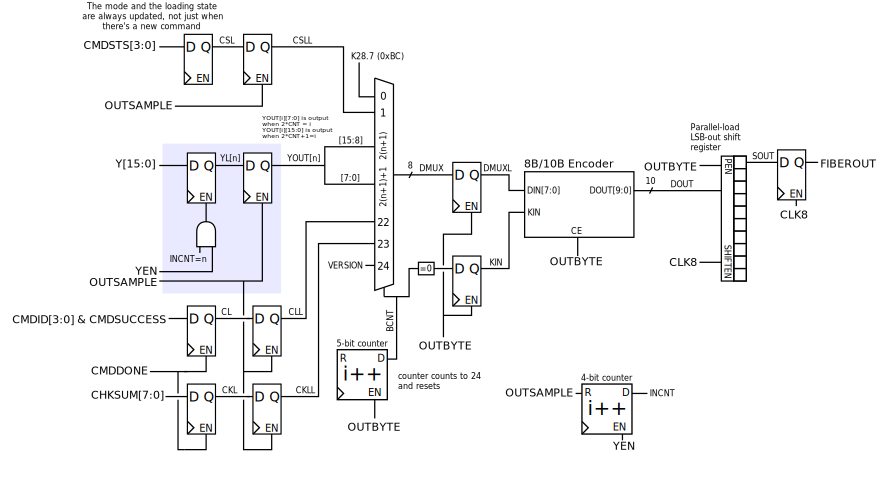
\includegraphics[scale=0.7]{fiberTX.svg}
\label{fibertx}
\caption{The Fiber Transmission interface}. 
\end{figure}
